% Chapter Template

\chapter{Experimental Results} % Main chapter title

\label{chp:results} % Change X to a consecutive number; for referencing this chapter elsewhere, use \ref{ChapterX}
In this chapter proposed methodologies are evaluated and compared with the related work.

All models are Trained using QaTa-Cov-19 \cite{ahishali2021advance} dataset using NVIDIA Tesla P-100 GPU and programmed using PyTorch.
\section{QaTa-COV19 Dataset}
\begin{center}
    \begin{figure}[htbp]
    \centerline{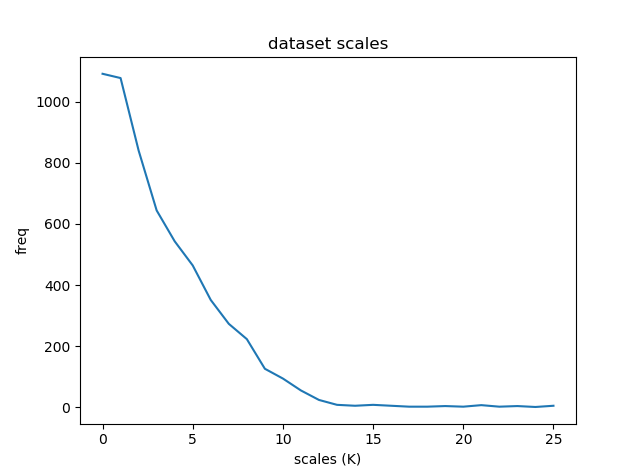
\includegraphics[height=60mm,width=9cm]{ScaleDist.png}}
    \caption{Pneumonia Scales of QaTa-COV19-v1, Y-axis represents the frequency, number of occurrence, of a pneumonia with a particular area}
    \label{pdist}
    \end{figure}
    \end{center}
QaTa-COV19 is a benchmark dataset for COVID19 detection and Segmentation form CXR images. All models that used for comparison are trained using QaTa-COV19-v1. Qata-COV19-v1 consist of  4603 COVID-19 CXR and  and $120,013$ control group CXRs. A balanced number of samples for the two classes is used, namely 4603 CXR image for each class to train the models. Pneumonia Scales of QaTa-COV19-v1 does not exhibit a uniform distribution. Scale of the Pneumonia can be defined as number, area, of 8-neighbor connected pixels labeled as COVID19 pneumonia. QaTa-COV19-v1 provides a binary masks of 2951 COVID19 CXR image which can be used for approximating the distribution of scales across the data set. Fig. \ref{pdist} illustrates the statistical distribution of QaTa-COV19 scales. The non-uniform distribution of the scales allows the CNN models to only recognize the small scales and not a large scales.

\section{Evaluation of the Methodology I}


Experiments are conducted on a Lenovo Z50-70 with Intel CORE i7-4510U CPU 2.00 GHz, 8GB RAM, NVIDIA GeForce 840M GPU; and with python and PyTorch library.

\subsection{Details of the Proposed Architecture}
The Proposed architecture composed Convbase and Densebase . Convbase is composed of a $6$ feature extraction modules \textit{(FX)} preceded by batch normalization layer as shown in Fig.5. Each FX module can be considered sub-sequential model consists of RSB layer followed by Batch Normalization, Max-pooling and LeakyReLU activation function. The Densebase is a two fully connected layers that classify the Convbase output.


\subsection{Hyperparameter Specification}
All input  chest X-Ray images are resized to be 200 $\times$ 200. After resizing the input images, these images are fed the Convbase model part which consists of 6 layers of residual separated block. Each residual separated block is followed with batch normalization and LeakyReLU \cite{he2015delving} as activation function  as shown in. The output depth of each  residual separated block is 4$\times$16, 4$\times$32, 4$\times$64, 4$\times$64, 4$\times$64 and 4$\times$16, respectively. The output of Convbase model part is 1D feature vector of 576 length. Densebase model part consists of two hidden layers. Each layer has the  size of 64 and the output layer of size 2. Each layer of Densebase layers is fully connected to its previous layer. The activation function used in the densebase model part is LeakyReLU. Table \ref{lyrSpec} summarizes the architecture hyperparameters.

\begin{table}[htbp]
\caption{The proposed architecture hyperparameters}
\begin{center}

\begin{tabular}{|l|c|c|}
\hline
\textbf{Layer Number} & \textbf{Layer Size} & \textbf{Activation Function} \\
\hline
\hline
RSBLayer1 & 4 $\times$ 16 & LeakyReLU\\
\hline
RSBLayer2 & 4 $\times$ 23 & LeakyReLU\\
\hline
RSBLayer3 & 4 $\times$ 64 & LeakyReLU\\
\hline
RSBLayer4 & 4 $\times$ 64 & LeakyReLU\\
\hline
RSBLayer5 & 4 $\times$ 64 & LeakyReLU\\
\hline
RSBLayer6 & 4 $\times$ 16 & LeakyReLU\\
\hline
\multicolumn{3}{|c|}{\textit{Flatten The Feature maps to 1D 576 feature  vector}}\\
\cline{1-3}
LinearLayer1 & 64 & LeakyReLU\\
\hline
LinearLayer2 & 64 & LeakyReLU\\
\hline
LinearLayer3 & 2 & Softmax\\
\hline
\end{tabular}
\label{lyrSpec}
\end{center}
\end{table}

\subsection{Network Training}
The proposed CNN model  is trained for 22 epoch. Adaptive Moment Estimation (Adam) optimizer \cite{kingma2014adam} is a popular optimization  technique for training deep networks. Adam optimizer is used  during the training  phase of the proposed CNN model. Both batch size and Adam optimizer learning rate is changed during the training phase if the training loss stopped decreasing. Table \ref{tabTrparam} summarizes the  parameters values used in the training phase of the proposed CNN model.  Fig. \ref{fig5}(a) show the progress for training and validation loss across each epoch. The difference between the training loss and validation loss through epochs show that our did not memorize the dataset.
\begin{table}[htbp]
\caption{The change of batch size and learning rate through the Training process}
\begin{center}

\begin{tabular}{|l|c|c|}
\hline
\textbf{Epoch Number} & \textbf{Batch Size} & \textbf{Learning Rate} \\
\hline
\hline
From 0 to 6 & 128 & 1e-3\\
\hline
From 7 to 12 & 256 & 1e-3\\
\hline
From 13 to 21 & 256 & 1e-4\\
\hline
 
\end{tabular}
\label{tabTrparam}
\end{center}
\end{table}



\subsection{Model Evaluation}

To assess the efficiency of the proposed method,  the proposed method is compared to recent state-of-the-art methods for detecting Covid-19 cases. Experiments are conducted with the same dataset and the corresponding hyperparameter of each work. All the methods depend on CNN. The comparison is performed using precision, sensitivity, F1-score, and accuracy \cite{hossin2015review}. In addition, the number of the parameters used in the training phase is  very important comparison factor. Table \ref{modelperf} depicts the comparison between state-of-the-art methods and the proposed method. As shown in the comparison, the proposed method  outperforms other methods achieving the maximum accuracy and the lowest  parameter count. 



\begin{table}[htbp]
\caption{ A performance comparison between the proposed method and state-of-the-art models.}
\begin{center}
\begin{tabular}{|l|c|c|c|c|c|}
\hline
\textbf{Method} & \textbf{PC} & \textbf{P(\%)}& \textbf{S(\%)}& \textbf{F1(\%)}& \textbf{A(\%)} \\
\hline
\hline
Proposed Method & 0.15M & 100.00 & 100.00 & 100.00 &100.00\\
\hline
ResNet-34 \cite{nayak2021application} & 21.8M & 96.77& 100.00 & 98.36 &98.33  \\
\hline
ACoS Phase I \cite{chandra2021coronavirus}& - & 98.266 & 96.512 & 98.551 & 98.062 \\
\hline
ResNet-50 \cite{nayak2021application}& 25.6M& 95.24& 100.00& 97.56& 97.50 \\
\hline
GoogleNet \cite{nayak2021application}& 5M &96.67& 96.67& 96.67& 96.67 \\
\hline
VGG-16 \cite{nayak2021application}& 138M& 95.08 & 96.67 & 95.87 &95.83\\
\hline
AlexNet \cite{nayak2021application}& 60M& 96.72 &98.33 & 97.52& 97.50 \\
\hline
MobileNet-V2 \cite{nayak2021application} & 3.4M &98.24& 93.33& 95.73 & 95.83 \\
\hline
Inception-V3 \cite{nayak2021application}& 24M &96.36& 88.33 & 92.17& 92.50\\
\hline
SqueezeNet \cite{nayak2021application}& 1.25M &98.27 &95.00& 96.61& 96.67 \\
\hline
\multicolumn{6}{l}{\textit{ PC is Parameter count, P is precision, S is sensitivity }}\\
\multicolumn{6}{l}{\textit{  F1 is F1-score, and A is accuracy }}\\
\hline
\end{tabular}
\label{modelperf}
\end{center}
\end{table}


\begin{figure}
\begin{center}
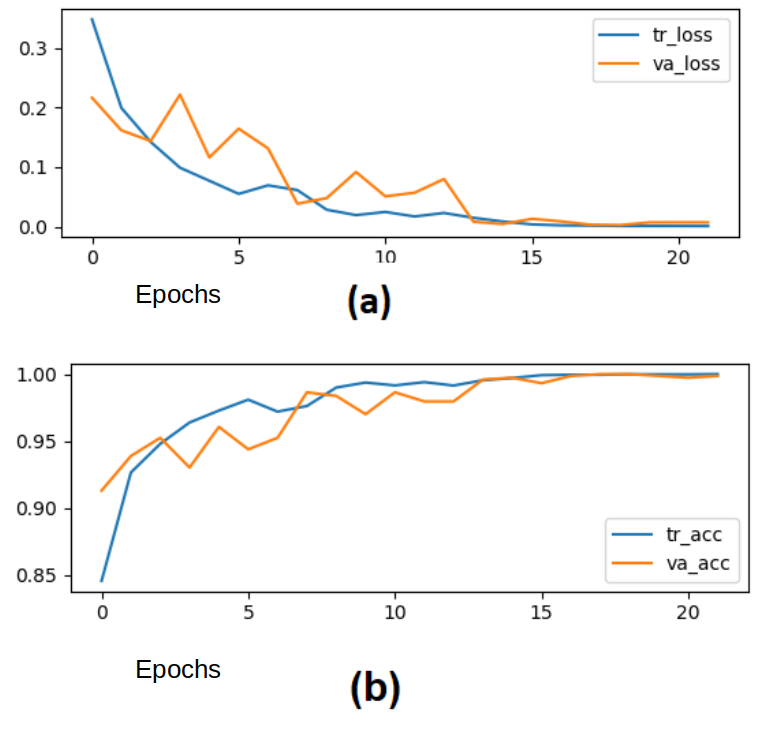
\includegraphics[height=90mm,width=8.0cm]{Figures/fig6.png}
\caption{(a) The training loss and the validation loss of each epoch and (b) The training accuracy and the validation accuracy of each epoch.}\label{fig5}\end{center}\end{figure}



\section{Evaluation of the Methodology II}
Methodology II is evaluated and compared against strong baselines and related works. 

\subsection{Baseline Networks}
Different architectures are trained to validate the effectiveness of the proposed method. 
\subsubsection{Spatial Pyramid Pooling (SPP-net) Based model}
A $4$ variants of SPP-net\cite{he2015spatial} is trained. All $4$ variant have the same architecture but different SPP-layer. These variants of SPP-layer are a full pyramid SPP of a 8-levels using average-pooling as aggregation function, full SPP pyramid of a 8-levels using max-pooling as aggregation function, single level SPP with 10-bins using average-pooling as aggregation function and single level SPP with 10-bins using max-pooling as aggregation function. A Fixed Architecture is used for all SPP variant models with the same design principles of the proposed architecture. This architecture is same as the proposed a architecture but DSWASPP is replaced by DC6 and SPP-1 layer is replaced with the corresponding SPP layer. DC6 is defined as six convolutional layer Densely connected together. For a SPP-net variants training a multiscale augmentation is added to the proposed augmentation process. multiscale augmentation is done by randomly sampling different $5$ scales typically $\{320, 320\pm25, 320\pm50 \}$.
\subsubsection{Switchable Atrous Spatial Pyramid Pooling (SASPP-net) Based models} 
\begin{center}
    \begin{figure*}[htbp]
    \centerline{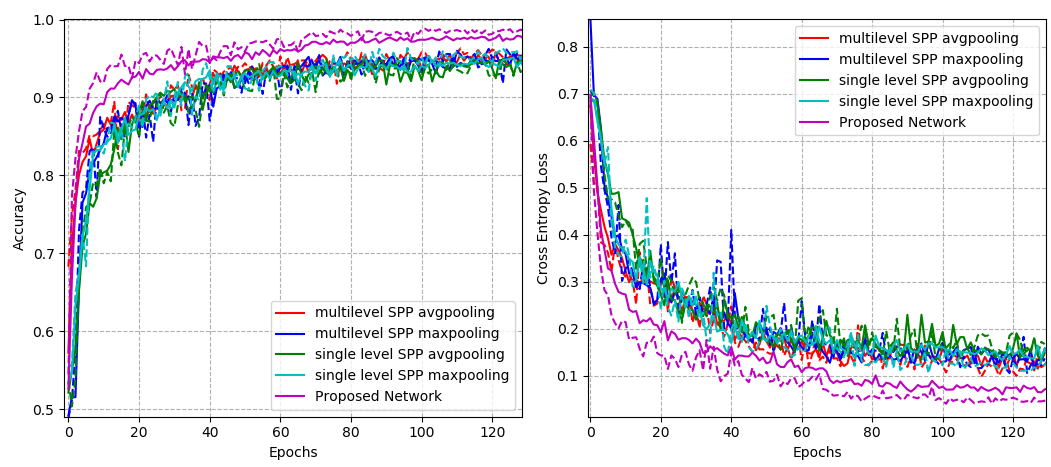
\includegraphics[height=63mm,width=15cm]{SPP-netsTraining.PNG}}
    \caption{Training profiles of both SPP-net variants and the proposed network. For the same color solid line represent training statistics while dashed line represent the validation statistics for the corresponding model. \textbf{left:} is the training accuracy. \textbf{Right:} is the training loss.}
    \label{SPP-train}
    \end{figure*}
    \end{center}
Another Base-line is introduced for comparison which is exactly as same as the proposed network but with different Attention module structure and does not includes a bottleneck within ASPP. This architecture is referred Switchable Atrous Spatial Pyramid Pooling (SASPP-net). Attention module structure is $Softmax(FC(GAP(X)))$ where: \textit{$X$: is the input feature map}, \textit{$GAP$: is a global average pooling},  \textit{$FC$: is fully Connected layer performs a non-linear projection to ${\rm I\!R}^{4}$ a 4 values for the three scales and the input feature map}.\\

\begin{table}[htbp]
\caption{}
\begin{center}
\begin{tabular}{|c|c|c|}
\hline
\textbf{Model}&\multicolumn{2}{|c|}{\textbf{Baseline CNN Architectures}} \\
\cline{2-3} 
\textbf{Type} & \textbf{\textit{Variant}}& \textbf{\textit{Param. Count}} \\
\hline
  & ML Average pooling & $14,916,420$   \\
\cline{2-3} 
SPP & ML max pooling & $14,916,420$   \\
\cline{2-3} 
  & SL Average pooling & $14,490,436$   \\
\cline{2-3} 
  & SL max pooling & $14,490,436$ \\
\hline
\multicolumn{2}{|c|}{SASPP} & $13,031,841$\\
\hline
\multicolumn{3}{l}{ \textbf{ML}: Multilevel, \textbf{SL}: Single level}
\end{tabular}
\label{Basarch}
\end{center}
\end{table}
Table \ref{Basarch} summarizes the base-line models and the Corresponding parameter count.
\subsection{Models Training}
Proposed architecture and baseline architecture are trained with the same hyperparameters. Dataset is split to $0.6$, $0.2$ and $0.2$ for training, validation and testing, respectively. For training a Cross Entropy Loss is used. All models trained with ADAM \cite{kingma2014adam} optimizer with learning rate start by $10^{-3}$ and reduced every time validation loss plateau by multiplying by $10^{-1}$. A Max Norm Constraint is used to clip the gradient value to norm of $1$ \cite{krizhevsky2012imagenet}. A batch size of $128$ is used to calculate the gradient.
\subsection{Reducing the overfitting}
overfitting is a critical problem for training large networks \cite{krizhevsky2012imagenet}. Proposed work has reduced the overfitting by using:
\begin{itemize}
\item Using Dropout with a retrain probability of $0.5$ \cite{srivastava2014dropout}.
\item Using BatchNorm adds noise due to randomization introduced when constructing the minibatch \cite{ioffe2015batch}.
\item Using max norm constraint \cite{krizhevsky2012imagenet}.
\item deep and thin architectures by design has an implicit regularization effect \cite{he2016deep}. 
\item Augmentation process i.e.) Texture augmentation \cite{krizhevsky2012imagenet}. 
\item The use of small kernel size \cite{simonyan2014very}.
\item bottleneck in SWASPP module and the attention module.
\end{itemize}
During training no overfitting effects is observed.
\subsection{comparison with baselines}
Proposed network is compared with the vanilla SPP-based Architectures and ASPP architecture.
\subsubsection{comparing with SPP-nets}
Fig. \ref{SPP-train} illustrates both training loss and training and validation accuracies and losses. Table \ref{blaccom} illustrates the testing accuracy for comparison between the SPP-nets baseline and the proposed architecture.


\begin{table}[htbp]
\caption{Comparison between Proposed network and baseline SPP architectures }
\begin{center}
\begin{tabular}{|c|c|}
\hline
\textbf{Model Name}& Accurracy \\
\hline
 SPP ML Average pooling & $0.958$   \\
\hline
SPP ML max pooling & $0.950$   \\
\hline
  SPP SL Average pooling & $0.927$   \\
\hline
  SPP SL max pooling & $0.957$ \\
\hline
Proposed Network & $0.987$\\
\hline
\multicolumn{2}{l}{ \textbf{ML}: Multilevel, \textbf{SL}: Single level}
\end{tabular}
\label{blaccom}
\end{center}
\end{table}
\subsubsection{comparing with SASPP}
Fig. \ref{saspp} illustrates the training and validation loss of training a SASPP baseline architecture. As shown in Fig. \ref{saspp} SASPP unable to generalize and start overfitting the training set. This comparison empirically shows the importance of the bottleneck introduced in the proposed architecture.

\begin{center}
\begin{figure}[htbp]
\centerline{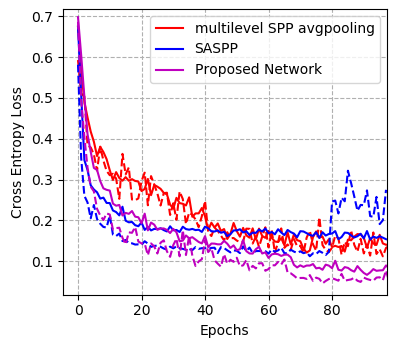
\includegraphics[height=55mm,width=8cm]{saspp.PNG}}
\caption{SASPP baseline architecture loss during both training, solid line, and validation, bashed line, compared with Proposed network and best performing SPP architecture.}
\label{saspp}
\end{figure}
\end{center}

\subsection{Comparing with the related works}
To fairly compare with the related works proposed work is further trained. Fig. \ref{ploss} shows the training and validation loss of the proposed network. Fig. \ref{pacc} shows the of the training and validation accuracy. 
\begin{center}
\begin{figure}[htbp]
\centerline{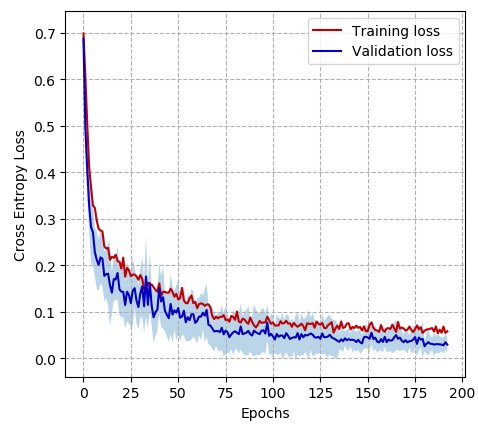
\includegraphics[height=55mm,width=8cm]{PLOSS.PNG}}
\caption{Cross entropy loss of the proposed architecture.}
\label{ploss}
\end{figure}
\end{center}
\begin{center}
\begin{figure}[htbp]
\centerline{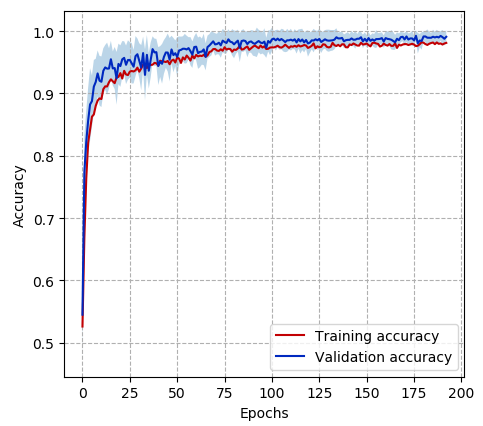
\includegraphics[height=55mm,width=8cm]{PACC.PNG}}
\caption{Training and validation accuracy of the proposed architecture.}
\label{pacc}
\end{figure}
\end{center}
Proposed Network has a sensitivity, recall, and precision of $0.994$ and $0.991$ respectively on the validation set. precision can be improved by investigating the precision-recall trade-off. Fig. \ref{prt} shows the trade-off between precision and recall for different thresholds. A threshold of $0.618$ is used to improve the precision resulting in a sensitivity, recall, of $0.9903$ and precision of $0.9956$.
Comparison metrics are defined as follow:
\begin{itemize}
\item \textit{Accuracy}: is ratio of correctly classified samples to the total number of samples
\item \textit{Sensitivity}: is ratio of correctly classified Covid-19 samples to the total number of actual Covid-19 samples 
\item \textit{Precision}: is the ratio of correctly, according to the ground-truth labels, classified Covid-19 samples to the total number of samples classified as Covid-19.
\item \textit{Specificity}: is the ratio of correctly, according to the ground-truth labels, classified non-Covid19 to the total number of non-Covid-19.
\item \textit{F1-score}: is the harmonic mean of both Sensitivity and Precision.
\begin{center}  
 $F_{1}=\frac{2\times\text{Precision} \times \text{Sensitivity}}{\text{Precision} + \text{Sensitivity}}$
\end{center}
\item \textit{Param. Count}: is the total number of the trainable parameters.
\end{itemize}


\begin{table*}[!p!t]
\caption{Comparison between Proposed network and Related works }
\begin{center}
\begin{tabular}{|c|c|c|c|c|c|c|}
\hline
\textbf{Model Name}& \textbf{Accuracy} & \textbf{Sensitivity} &\textbf{ Precision} & \textbf{Specificity} & \textbf{F1-score} & \textbf{Param. Count}\\
\hline
\hline
Proposed & 0.99294 & \textbf{0.9903} & \textbf{0.9956} & 0.9956 & \textbf{0.9929} & \textbf{5,040,571}\\
\hline
SRC-Dalm\cite{ar} & 0.985 & 0.886 & - & 0.993 & - & -\\
\hline 
SRC-Hom\cite{ar} & 0.977 & 0.921 & - & 0.982 & - & - \\
\hline
CRC-light\cite{ar} & 0.973 & 0.955 & - & 0.974 & - &- \\
\hline
DenseNet121*\cite{ar} & 0.992 & 0.9714 & - & 0.9949 & - & 6,955,906  \\
\hline
Inception-v3\cite{ar} & 0.993 & 0.954 & - & 0.998 & - & 21,772,450  \\
\hline
Modified MobileNetV2 \cite{akt}  & 0.98 & 0.98 & 0.97 & - & 0.97 & -\\
\hline
ReCovNet-v2\cite{dag} & 0.99726 & 0.98571 & 0.94262 & 0.9977 & 0.96369 &- \\
\hline
ReCovNet-v1\cite{dag} & 0.99824 & 0.9781 & 0.97438 & 0.99901 & 0.97624 & -\\
\hline
DenseNet-121\cite{dag}  & \textbf{0.9988} & 0.97429 & 0.9932 & \textbf{0.99974} & 0.98365 & 6,955,906 \\
\hline
\end{tabular}
\end{center}
\label{rwcom}
\end{table*}


\begin{center}
\begin{figure}[htbp]
\centerline{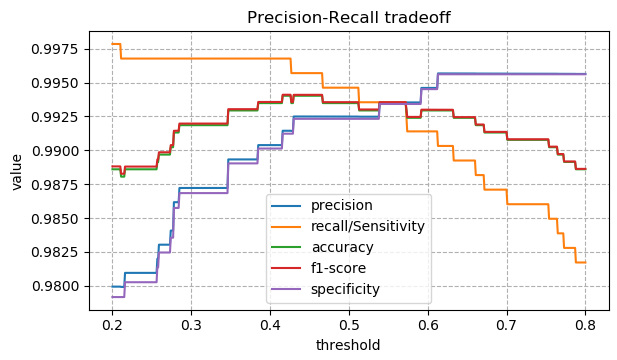
\includegraphics[height=55mm,width=8cm]{PresRecuTradff.PNG}}
\caption{precision-recall trade-off of the proposed network.}
\label{prt}
\end{figure}
\end{center}


Table \ref{rwcom} summarizes the comparison between the recent related works and the proposed architecture. Proposed architecture outperform these works in many metrics. As their training and testing does not depend on a balanced number of samples, accuracy and specificity are not good metrics for  evaluation. 
